\documentclass[10pt,conference,compsocconf]{IEEEtran}

\usepackage{hyperref}
\usepackage{graphicx}	% For figure environment
\usepackage{amsmath}
\usepackage{amssymb}
\usepackage{float}
\usepackage{url}
\newcommand{\beginsupplement}{%
	\setcounter{table}{0}
	\renewcommand{\thetable}{S\arabic{table}}%
	\setcounter{figure}{0}
	\renewcommand{\thefigure}{S\arabic{figure}}%
}

\begin{document}
\title{Extreme Wind Analysis}

\author{
	Matthias Minder, Yves Rychener
}

\maketitle

\begin{abstract}

\end{abstract}

\section*{Introduction} 
Modeling extreme weather events is of interest for a variety of applications, such as risk assessment for insurance companies or conception of preventive measures. In particular, questions about how often a particular event will occur, how severe events can get, and whether there are seasonal or year-dependent trends are of interest. Within the scope of this report, we will address these questions for extreme thunderstorms on a 1° longitude and 1° latitude grid cell with south-west coordinates 38° latitude and -100° longitude, situated in central Kansas. The measured quantities are the Connective Available Potential Energy ($CAPE$) and the Storm Relative Helicity ($SRH$), which have to be simultaneously high for severe thunderstorms to occur. Three-hourly time series of these events are taken into account from January 1st 1979 at 00:00 to December 31st 2015, 21:00. 
\par
In particular, we will study the value denoted $PROD$ given by $PROD = \sqrt{CAPE} \times SRH$. It captures concurrently high values of $SRH$ and $CAPE$, and is thus apt for modeling the risk of thunderstorms. Every month will be treated separately in order to capture seasonal differences. To model extreme values, a generalized extreme value distribution will be fitted to the monthly maxima of $PROD$ using maximum likelihood estimation as well as Bayesian approaches. Moreover, the generalized extreme value distribution will be fitted to the $r$-largest order statistic for every month to determine whether that improves the fit. Subsequently, we will assess dependence of $PROD$ upon time and the NINO 3.4 index, an established indicator of the El-Niño Southern Oscillation ($ENSO$). 
\par
Following this, $CAPE$ and $SRH$ are considered separately. We will study whether they are asymptotically dependent, before fitting bivariate models to the joint extremes of $CAPE$ and $SRH$. 
Finally, 50- and 100-year return levels of $PROD$ are calculated based on fitting a point process model to $PROD$ with maximum likelihood estimation, based on the Bayesian fit, and based on simulated values of $CAPE$ and $SRH$ from the bivariate model fitted before. 

\section*{Preliminary Analysis}
\begin{figure}
	\centering
	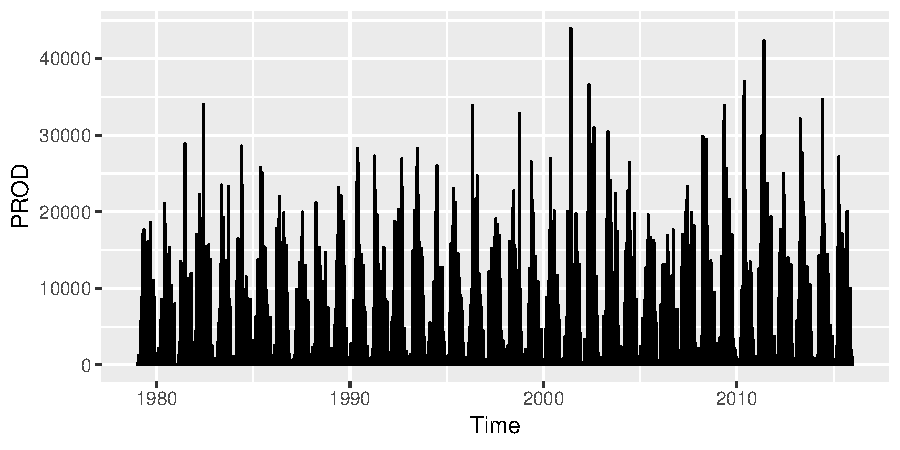
\includegraphics[width=0.35\textwidth]{../plots/full_time_series.pdf}
	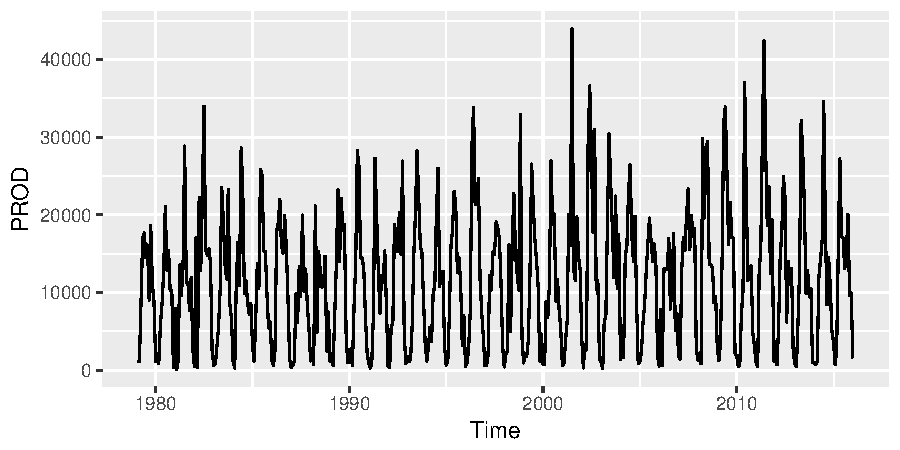
\includegraphics[width=0.35\textwidth]{../plots/monthly_max_series.pdf}
	\caption{Three-hourly values (top) and monthly maxima (bottom) of $PROD$ values for the entire analyzed period.}
	\label{fig:timeseries}
\end{figure}
Plotting the full time series and the monthly maxima as shown in Figure \ref{fig:timeseries} clearly shows the seasonality of the data, with high values of $PROD$ occurring mainly during summer. This clearly shows the necessity of separate treatment of months. Moreover, there seems to be some upward trend following time, with more extreme values of $PROD$ in recent years.

\section*{Fitting Generalized Extreme Value Distribution to PROD}
In order to understand the behavior of the monthly maxima, we fitted a generalized extreme value (GEV) distribution to $PROD$ for each month separately with three different approaches. 
\begin{figure}
	\centering
	\textbf{January}\\
	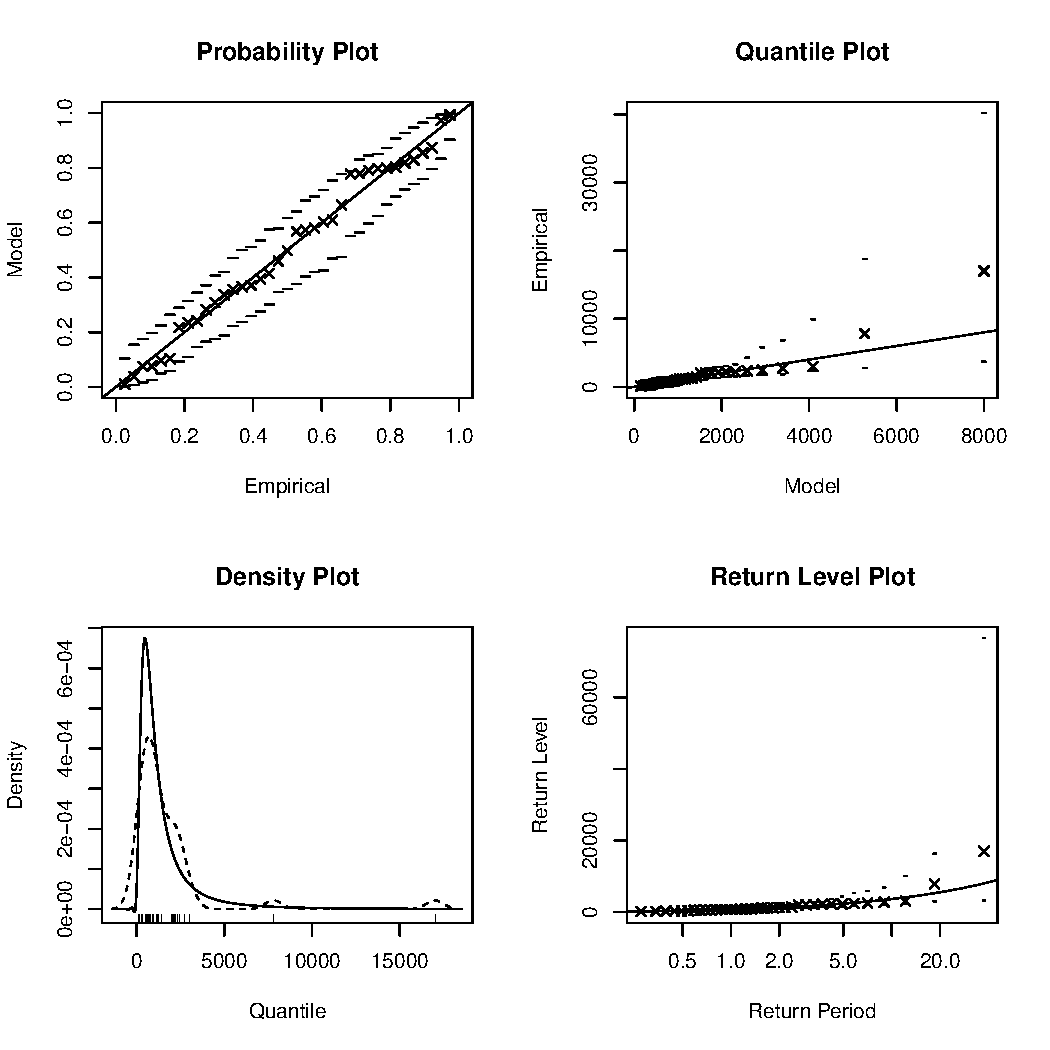
\includegraphics[width=0.35\textwidth]{../plots/monthly_mle_diag/01_monthly_mle_diag.pdf}\\
	\textbf{December}\\
	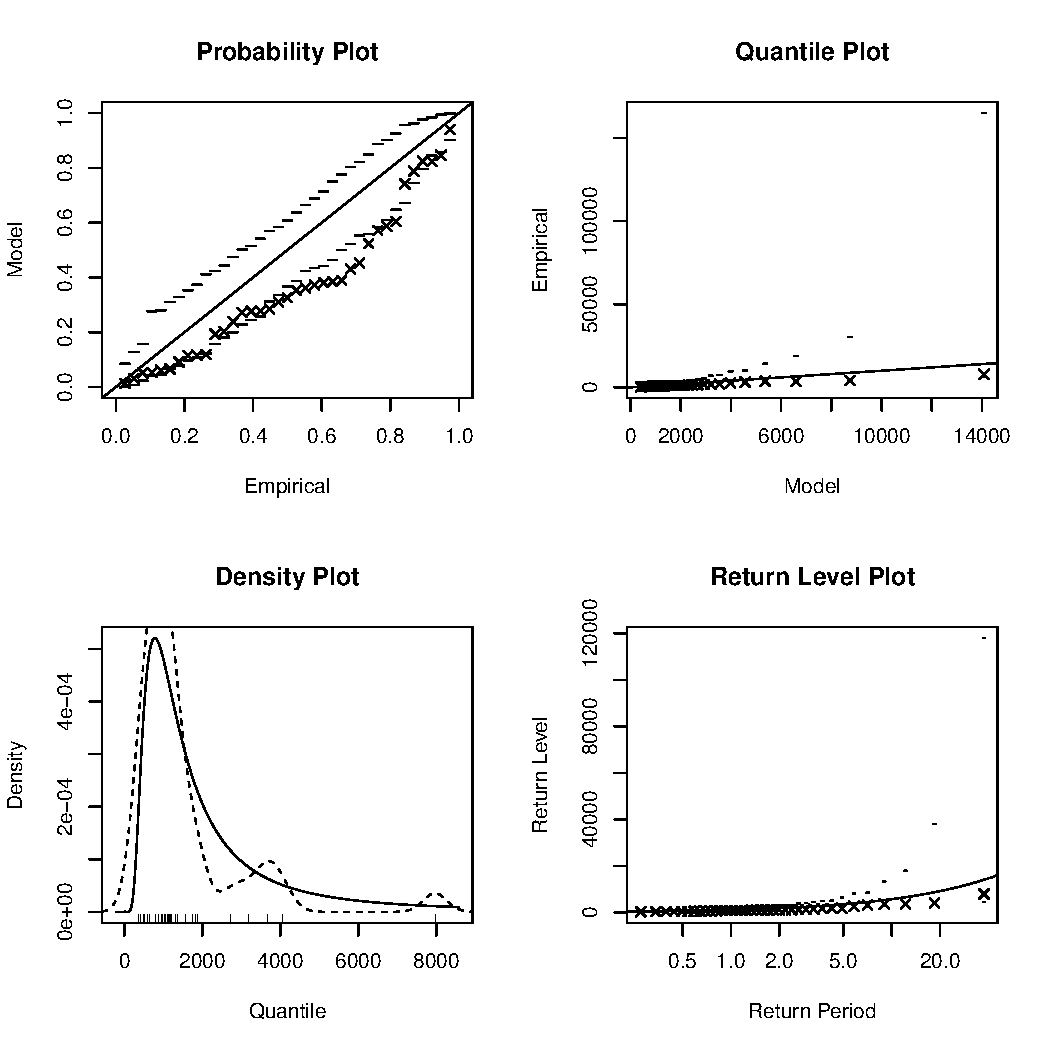
\includegraphics[width=0.35\textwidth]{../plots/monthly_mle_diag/12_monthly_mle_diag.pdf}
	\caption{Diagnostic plots for fitting GEV to the data using maximum likelihood estimation for January (top) and December (bottom). Whereas in January the model fits the data, as shown by the fact that the observed values are within the confidence range for probability plot, this is not the case for December, indicating a poor fit.}
	\label{fig:mle_diag}
\end{figure}
\par
First, we fitted the values using maximum likelihood estimation. Fitting was done using the evd package in R, using the Nelder-Mead optimization method and standard parameters \cite{evd}. The quality of the fit was assessed using diagnostic plots, as shown for January and December in Figure \ref{fig:mle_diag}. The model performed well with the exception of September and December: In September optimization didn't succeed, whereas in December the observed values lie outside of the given confidence intervals, as shown in Figure \ref{fig:mle_diag}. For both of these months, no standard error could be calculated due to singularity of the observed Fisher information matrix. Since we expect some continuity over the course of the year, the problem wasn't further investigated as inferences for the missing months can be made from their adjacent months. 

\section*{Dependence of PROD on Time and ENSO}


\section*{Dependence of CAPE and SRH}


\section*{Bivariate Fitting of CAPE and SRH}


\section*{Calculation of Return Levels}

\section*{Conclusion}



%%% Bibliography
\bibliographystyle{IEEEtran}
\bibliography{literature-project}


	
\end{document}
